% 8장 가격은 잡혔나. 0001 · 0003 · 0018 · 0025 · 0026

\section{가격은 잡혔나}

토허제의 명분이 가격 안정이므로 이 장이 제도 평가의 직접적인 자리다. 결론을 먼저
적으면 \textbf{가격을 잡았다는 증거는 약하다.}

\subsection{구성 변화 문제}

거래가 80\% 줄면 \textbf{팔리는 집의 종류가 바뀐다.} 어느 동의 한 달 평균 가격은
그달에 팔린 집들의 평균이므로, 각 단지의 가격이 하나도 변하지 않아도 어떤 단지가
더 많이 팔렸느냐에 따라 평균이 움직인다. 측정된 ``평균 가격 변화'' 안에
\textbf{진짜 가격 변화 + 구성 변화}가 섞인다.

구성이 실제로 바뀌었다. 처치동 사후 표본의 평균 전용면적이 93.9\,m$^2$에서
88.7\,m$^2$로 이동했고, 2020년 9월에는 처치 4개 동의 월평균 전용면적이
103.4\,m$^2$로 튀면서 그달의 중위가 지수(170.5)와 반복매매지수(159.4)가
\textbf{11포인트} 벌어졌다.

\subsection{지수 다섯의 사다리}

구성 통제의 사다리로 같은 자료에 지수 다섯을 지었다(3.4절, 0025). 아래로 갈수록
더 많은 것을 고정한다. 지정 전후 12개월, 처치동 $\div$ 통제동 비의 변화다.

\begin{table}[htbp]
  \centering
  \caption{무엇을 고정하느냐에 따라 가격 효과가 절반이 된다}
  \label{tab:price-ladder}
  \begin{tabular}{llr}
    \toprule
    \textbf{가격지수} & \textbf{무엇을 고정하나} & \textbf{12개월 변화} \\
    \midrule
    중위가 (총액) & 아무것도 & $-10.1\%$ \\
    중위가 (㎡당) & 물건의 크기 & $-12.5\%$ \\
    헤도닉 & 면적과 층 & $-11.1\%$ \\
    \textbf{헤도닉 + 단지} & 거기에 단지의 질까지 & $\mathbf{-5.9\%}$ \\
    \textbf{반복매매} & 같은 집 & $\mathbf{-6.0\%}$ \\
    \bottomrule
  \end{tabular}
\end{table}

\begin{figure}[htbp]
  \centering
  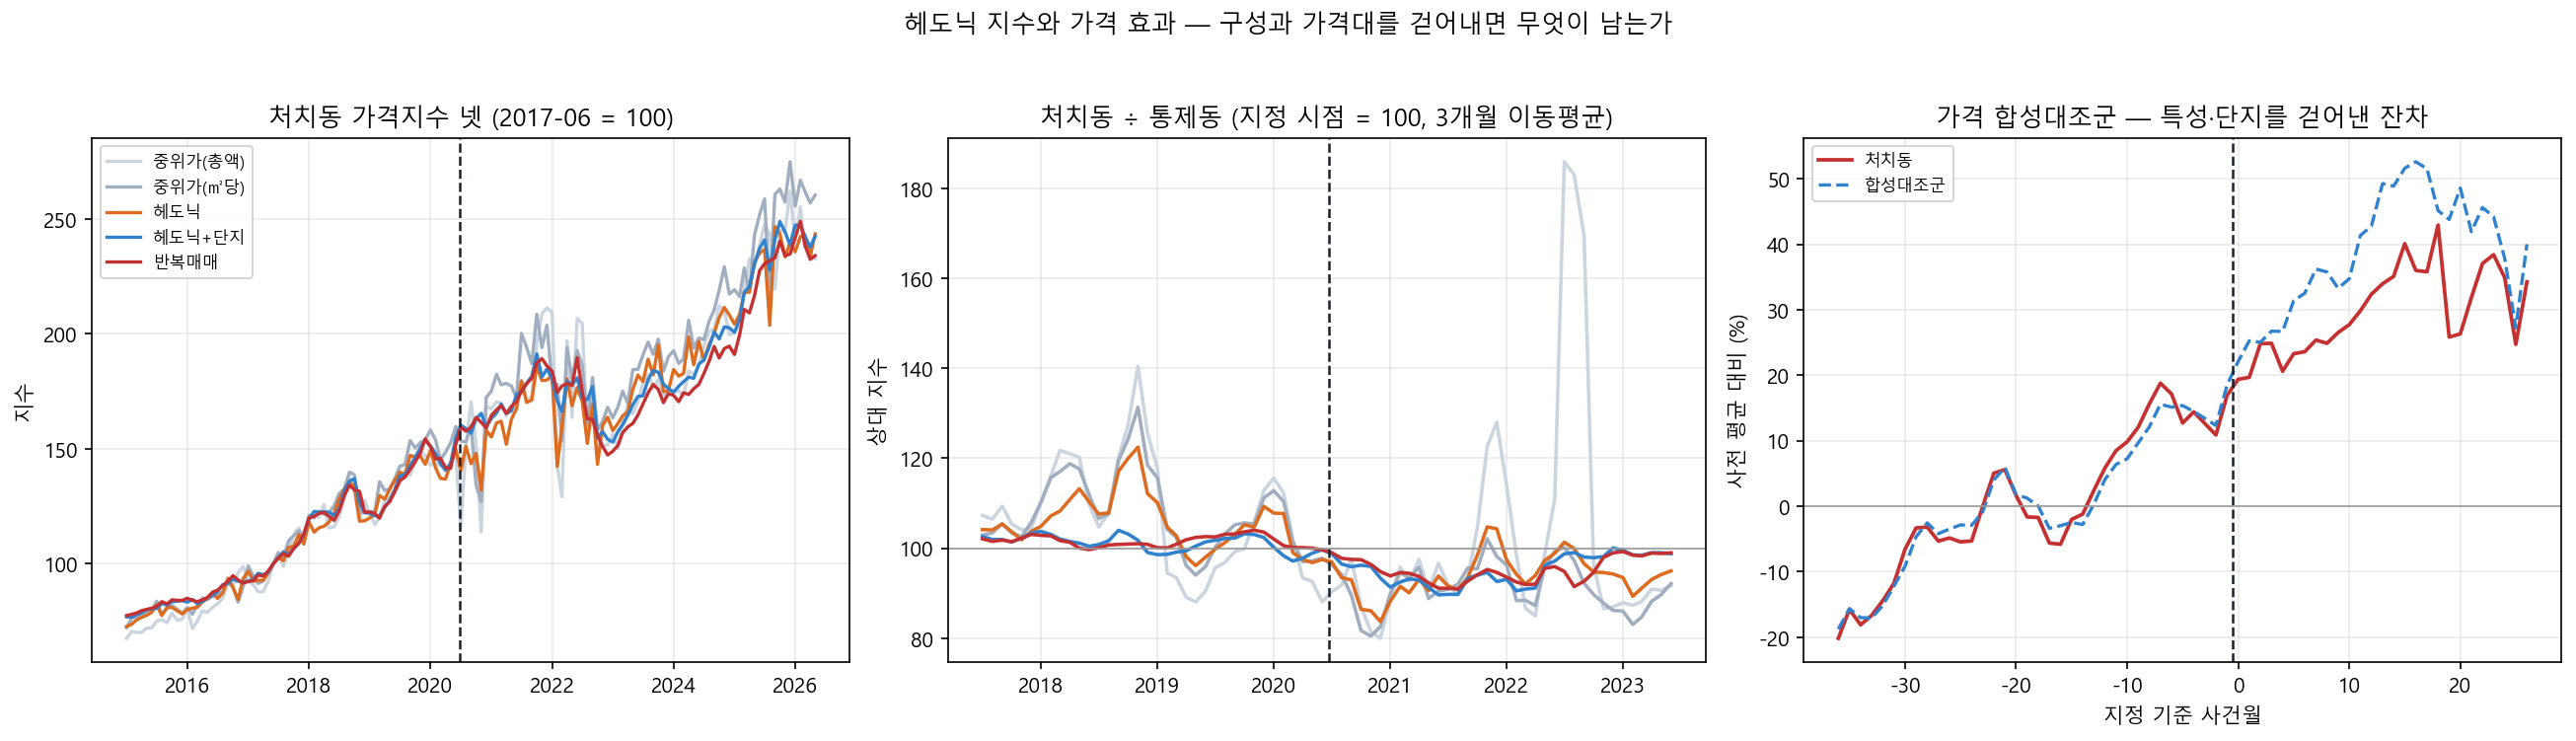
\includegraphics[width=\linewidth]{08_hedonic.png}
  \caption{가격지수 다섯과 통제군 격자.}
  \label{fig:hedonic}
\end{figure}

\textbf{결정적인 칸은 단지 고정효과다.} 면적·층만 통제하면 $-11.1\%$인데 어느
단지의 집이 팔렸는지까지 고정하면 $-5.9\%$로 절반이 된다. \textbf{집계 지수의
$-10 \sim -12\%$는 절반쯤이 구성 변화였다.}

그리고 \textbf{약점이 정반대인 두 방법이 $-5.9\%$와 $-6.0\%$에서 만난다.}
반복매매는 두 번 팔린 집만 쓰고(선택편의), 헤도닉은 모든 거래를 쓰되 관측되는
특성만 통제한다. 둘이 일치하면 서로를 떠받친다.

\subsection{통제군 격자}

통제군을 바꾸면 값이 흔들린다. 같은 창, 같은 지수로 통제군 둘 $\times$ 사양 넷을
돌렸다.

\begin{table}[htbp]
  \centering
  \caption{통제군을 바꿀 때 (12개월 변화)}
  \label{tab:price-grid}
  \begin{tabular}{lrrrr}
    \toprule
    \textbf{통제군} & \textbf{중위 총액} & \textbf{중위 ㎡당} &
    \textbf{헤도닉} & \textbf{헤도닉+단지} \\
    \midrule
    강남·송파 통제동 & $-5.5\%$ & $-6.7\%$ & $-4.2\%$ & $-5.9\%$ \\
    서울 나머지 19개 구 & $-9.8\%$ & $-10.7\%$ & $\mathbf{-2.1\%}$ &
      $-4.2\%$ \\
    \bottomrule
  \end{tabular}
\end{table}

처치동 아파트는 서울 최상위 가격대에 몰려 있고 2020$\sim$2021년은 중저가가
급등하고 고가가 뒤처진 시기다. 그래서 지정 전 ㎡당가가 처치동 범위에 드는 단지만
남긴 \textbf{공통지지} 표본에서는 가격 효과가 $-2.1\%$($p=0.270$)로 약해진다.

\textbf{읽는 방법이 둘이다.} 토허제의 가격 효과로 보였던 것이 사실은 2020$\sim$21년
고가 단지가 뒤처진 것일 수 있고, 반대로 규제가 고가 단지에 걸렸으니 가격대를
맞추는 것은 처치의 일부를 빼는 것일 수 있다. \textbf{지금 자료로는 가르지 못한다.}

\textbf{버린 사양을 밝혀 둔다.} 가격대를 통제하려고 처음에는 가격 10분위 $\times$
시점 고정효과를 넣었다. 처치동 가격 효과가 $-1.0\%$까지 사라지길래 확인해 보니
\textbf{최상위 분위 거래의 20.3\%가 처치동이고, 처치동과 맞닿은 동을 합치면
49.4\%}였다. 처치가 제 통제군이 되어 효과를 기계적으로 흡수하는 구조다. 고정효과로
빼는 대신 표본을 줄여 비교 대상을 명시적으로 고르는 쪽으로 바꿨다.

\subsection{사전 추세를 열면 무너진다}

지금까지 사전 추세는 \textbf{진단}만 했다(4.5절). 기준 분기를 옮겨 보는 것은 대안
사양 몇 개를 보는 것이지 \textbf{위배의 크기를 모수로 놓고 푸는 것이 아니다.}

\citet{rambachan2023honest}는 평행추세를 성립/불성립으로 묻지 않는다. 사후에 남아
있을 수 있는 위배를 모수 $\bar{M}$ 하나로 제한하고, 그 모수를 키워 가며
\textbf{구간이 언제 0을 품는지}를 본다. 그 지점이 \textbf{붕괴값}이다.
$\bar{M}=1$은 ``사전에 가장 크게 흔들렸던 만큼이 사후에도 매 분기 그대로
이어졌다''는 뜻이다.

\begin{table}[htbp]
  \centering
  \caption{사전 추세를 열어 둘 때의 붕괴값}
  \label{tab:breakdown}
  \begin{tabular}{lr}
    \toprule
    \textbf{무엇을 재나} & \textbf{붕괴값 $\bar{M}$} \\
    \midrule
    \textbf{거래량 --- 지정 직후 3개월} & $\mathbf{1.62}$ \\
    거래량 --- 24개월 평균 & 0.05 \\
    \textbf{가격 --- 지정 후 12개월} & $\mathbf{0.22}$ \\
    \bottomrule
  \end{tabular}
\end{table}

\begin{figure}[htbp]
  \centering
  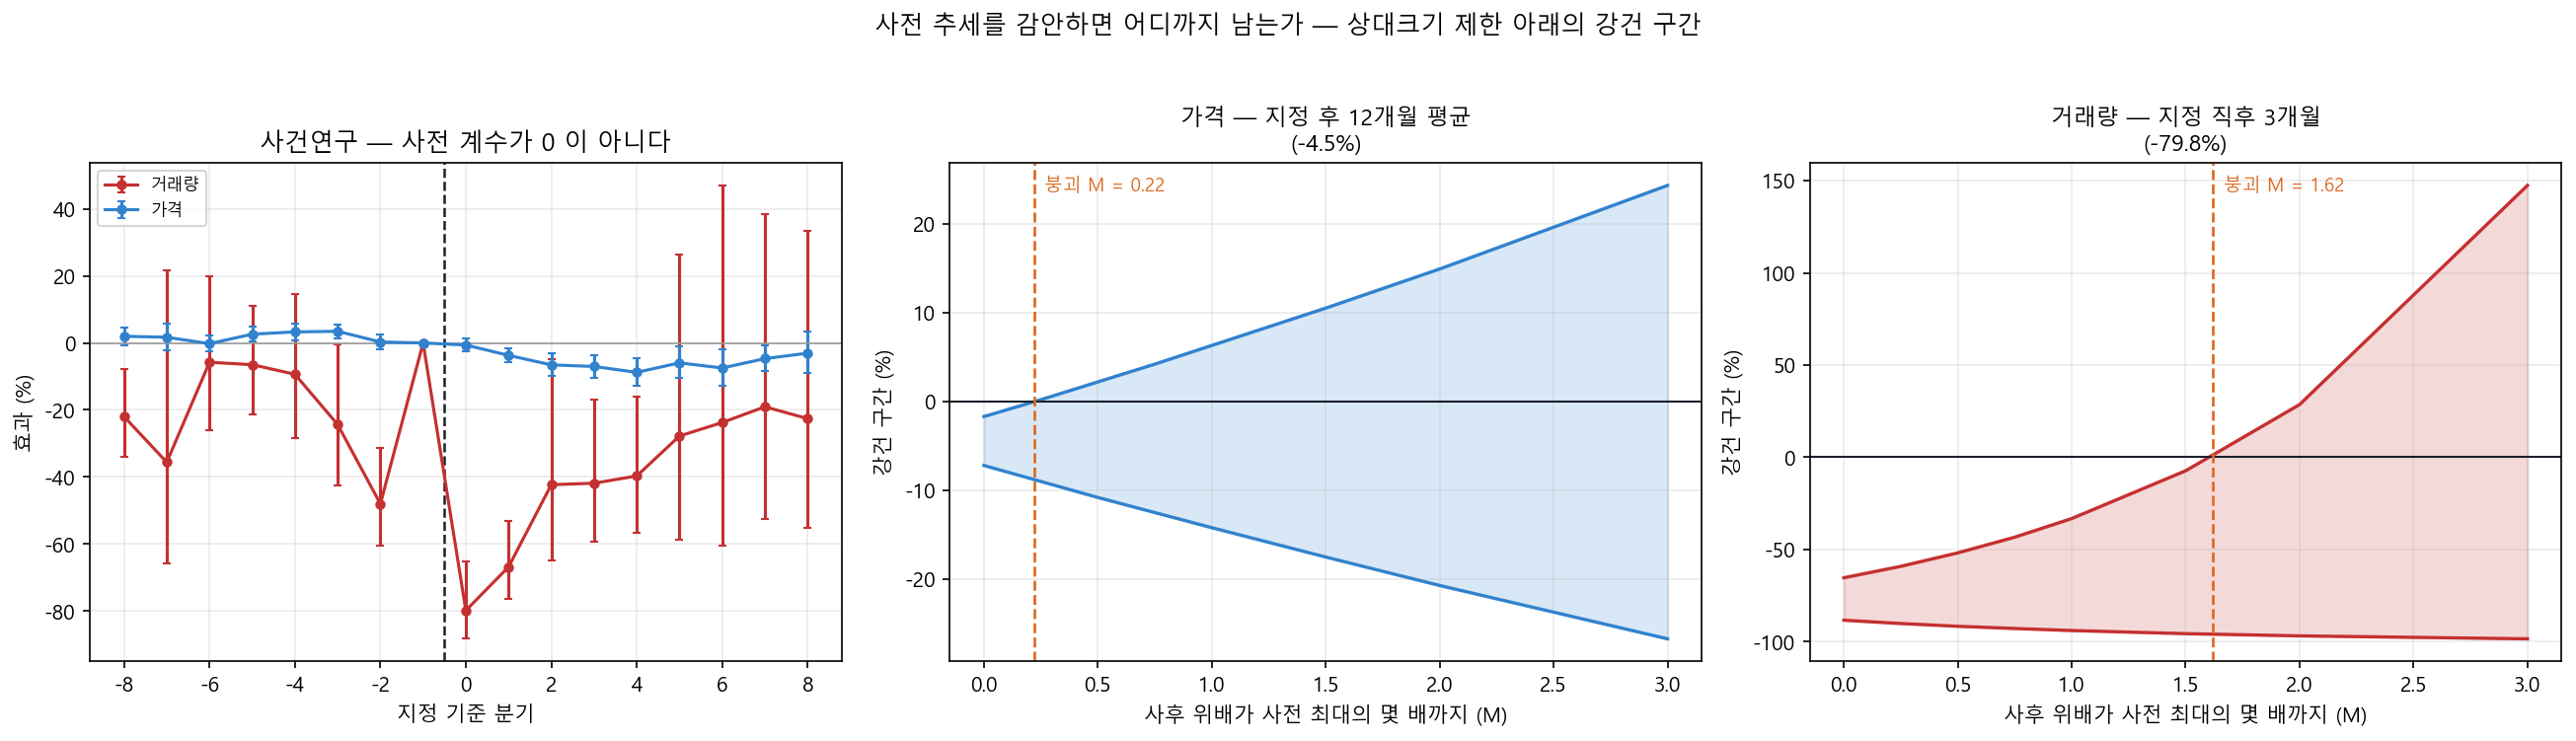
\includegraphics[width=\linewidth]{11_honest_did.png}
  \caption{사전추세 민감도 구간. $\bar{M}$ 을 키워 가며 구간이 0 을 품는 지점을
           본다.}
  \label{fig:honest-did}
\end{figure}

\textbf{거래량 직후 효과는 사전 위배의 1.6배까지 열어 두어도 남고, 가격은 0.22에서
무너진다.} 7분의 1이다. 가격 $-4 \sim -7\%$는 \textbf{평행추세를 가정했을 때만}
성립하는 값이다.

\subsection{합성대조군으로는 확인되지 않는다}

사람이 통제군을 고르지 않고 \textbf{사전 궤적이 가장 닮도록 자료가 가중치를 직접
찾게} 했다\citep{abadie2010synthetic}. 기증자 풀에서 맞닿은 동 14개는 뺀다 ---
7장에서 그 동들의 가격이 19개 구 대비 $-5.0\%$ 움직였으므로 파급을 받은 동을
통제군에 넣으면 효과가 0 쪽으로 끌린다(실제로 빼기 전 $-3.5\%$, 빼고 나서
$-5.1\%$).

\begin{table}[htbp]
  \centering
  \caption{합성대조군 --- 거래량과 가격}
  \label{tab:scm-compare}
  \begin{tabular}{llrr}
    \toprule
    \textbf{결과변수} & \textbf{검정 통계량} & \textbf{순위} &
    \textbf{경험적 $p$} \\
    \midrule
    거래량 & 지정 직후 3개월 ($-71.0\%$) & \textbf{1 / 152} &
      $\mathbf{0.007}$ \\
    거래량 & 사후 27개월 평균 ($-26.9\%$) & 22 / 152 & 0.145 \\
    가격 & 사후 12개월 평균 ($-5.1\%$) & 중간 & \textbf{0.511} \\
    \bottomrule
  \end{tabular}
\end{table}

\textbf{가격은 가짜 대치동 46개 가운데 중간쯤이다.} 우연과 구별되지 않는다.

\subsection{그래서 방향만 쓴다}

세 가지가 같은 방향을 가리킨다.

\begin{table}[htbp]
  \centering
  \caption{거래량과 가격 --- 같은 자료, 같은 사건, 같은 설계}
  \label{tab:vol-vs-price}
  \begin{tabular}{lrr}
    \toprule
    \textbf{검정} & \textbf{거래량} & \textbf{가격} \\
    \midrule
    설계 조합 중 유의하게 음수 & \textbf{192 / 192} & 70 / 144 \\
    붕괴값 $\bar{M}$ & \textbf{1.62} & 0.22 \\
    합성대조군 경험적 $p$ & \textbf{0.007} & 0.511 \\
    \bottomrule
  \end{tabular}
\end{table}

\textbf{그래서 가격은 ``내렸을 것이다''까지만 쓰고 ``몇 \% 내렸다''는 쓰지 않는다.}
설계를 바꿔 가며 144가지로 재면 $-18.2\%$에서 $+3.6\%$까지 움직이고 29개는 0 위로
올라간다. 거래량은 192가지 중 하나도 0을 넘지 않는다.

1주차에 주 결과변수를 가격에서 거래량으로 바꾼 것은 그때는 판단이었다(0001).
\textbf{다섯 달 뒤 세 가지 방법으로 그 결정이 확인됐다.}

\textbf{마지막으로 가격을 버리지 않은 이유를 적는다.} 선행연구 세 편이 모두 가격을
다루므로, 가격을 빼면 대조할 지점이 사라진다. 그리고 ``가격을 잡았다는 증거가
약하다''는 것 자체가 제도 평가의 결과다. 명분이 가격 안정인 제도에서 그 명분이
확인되지 않는다는 것은 \textbf{못 잰 것이 아니라 재서 알게 된 것}이다.
